\PassOptionsToPackage{unicode=true}{hyperref} % options for packages loaded elsewhere
\PassOptionsToPackage{hyphens}{url}
%
\documentclass[ignorenonframetext,]{beamer}
\usepackage{pgfpages}
\setbeamertemplate{caption}[numbered]
\setbeamertemplate{caption label separator}{: }
\setbeamercolor{caption name}{fg=normal text.fg}
\beamertemplatenavigationsymbolsempty
% Prevent slide breaks in the middle of a paragraph:
\widowpenalties 1 10000
\raggedbottom
\setbeamertemplate{part page}{
\centering
\begin{beamercolorbox}[sep=16pt,center]{part title}
  \usebeamerfont{part title}\insertpart\par
\end{beamercolorbox}
}
\setbeamertemplate{section page}{
\centering
\begin{beamercolorbox}[sep=12pt,center]{part title}
  \usebeamerfont{section title}\insertsection\par
\end{beamercolorbox}
}
\setbeamertemplate{subsection page}{
\centering
\begin{beamercolorbox}[sep=8pt,center]{part title}
  \usebeamerfont{subsection title}\insertsubsection\par
\end{beamercolorbox}
}
\AtBeginPart{
  \frame{\partpage}
}
\AtBeginSection{
  \ifbibliography
  \else
    \frame{\sectionpage}
  \fi
}
\AtBeginSubsection{
  \frame{\subsectionpage}
}
\usepackage{lmodern}
\usepackage{amssymb,amsmath}
\usepackage{ifxetex,ifluatex}
\usepackage{fixltx2e} % provides \textsubscript
\ifnum 0\ifxetex 1\fi\ifluatex 1\fi=0 % if pdftex
  \usepackage[T1]{fontenc}
  \usepackage[utf8]{inputenc}
  \usepackage{textcomp} % provides euro and other symbols
\else % if luatex or xelatex
  \usepackage{unicode-math}
  \defaultfontfeatures{Ligatures=TeX,Scale=MatchLowercase}
\fi
\usetheme[]{Antibes}
\usecolortheme{dolphin}
\usefonttheme{professionalfonts}
% use upquote if available, for straight quotes in verbatim environments
\IfFileExists{upquote.sty}{\usepackage{upquote}}{}
% use microtype if available
\IfFileExists{microtype.sty}{%
\usepackage[]{microtype}
\UseMicrotypeSet[protrusion]{basicmath} % disable protrusion for tt fonts
}{}
\IfFileExists{parskip.sty}{%
\usepackage{parskip}
}{% else
\setlength{\parindent}{0pt}
\setlength{\parskip}{6pt plus 2pt minus 1pt}
}
\usepackage{hyperref}
\hypersetup{
            pdfborder={0 0 0},
            breaklinks=true}
\urlstyle{same}  % don't use monospace font for urls
\newif\ifbibliography
\usepackage{longtable,booktabs}
\usepackage{caption}
% These lines are needed to make table captions work with longtable:
\makeatletter
\def\fnum@table{\tablename~\thetable}
\makeatother
\usepackage{graphicx,grffile}
\makeatletter
\def\maxwidth{\ifdim\Gin@nat@width>\linewidth\linewidth\else\Gin@nat@width\fi}
\def\maxheight{\ifdim\Gin@nat@height>\textheight\textheight\else\Gin@nat@height\fi}
\makeatother
% Scale images if necessary, so that they will not overflow the page
% margins by default, and it is still possible to overwrite the defaults
% using explicit options in \includegraphics[width, height, ...]{}
\setkeys{Gin}{width=\maxwidth,height=\maxheight,keepaspectratio}
\setlength{\emergencystretch}{3em}  % prevent overfull lines
\providecommand{\tightlist}{%
  \setlength{\itemsep}{0pt}\setlength{\parskip}{0pt}}
\setcounter{secnumdepth}{0}

% set default figure placement to htbp
\makeatletter
\def\fps@figure{htbp}
\makeatother

\useoutertheme{infolines}
\useinnertheme{circles}
\setbeamercolor{note page}{bg=white,fg=black}
\setbeamercolor{note title}{bg=white!80!black, fg=black}

\date{}

\begin{document}

\hypertarget{pareto-distribution}{%
\section{Pareto Distribution}\label{pareto-distribution}}

\begin{frame}{Background}
\protect\hypertarget{background}{}

\begin{itemize}
\tightlist
\item
  Vilfredo Pareto (1897) presents a versatile functional relation that
  well describes wealth distribution across countries and centuries.
\item
  Same concept is applied to several other fields and colloquially
  called \emph{Pareto Principle}.

  \begin{itemize}
  \tightlist
  \item
    80\% of land owned by 20\% of individuals (revenue \(\sim\)
    products; sales \(\sim\) clients; etc)
  \end{itemize}
\item
  Generally, it follows a \emph{power law probability distribution},
  where one measure varies constantly as an exponential of another,
  independently of initial values.

  \begin{itemize}
  \tightlist
  \item
    Example: if one increases the side length of a square by \(x\), its
    area increases by \(x^2\), independently of initial area of square.
  \end{itemize}
\end{itemize}

\note{\begin{itemize}\tightlist
\item
I am going to talk about the theoretical framework in our replication study. Since
the focus of the study is not only to provide new information, which is usually 
hard to come by, but also to check if we can make some more general inferences 
about  wealth distribution in germany and adapt the top tail of the SOEP accordingly. 
\item AS A BACKGROUND: Pareto (the same of the optimallity concept)
\item functional form that describes well the wealth distribution accross countries and time

\item an approximate description of the distribution of incomes and wealth among the rich and the moderately rich
\item 80/20 rule (revenue / sales; )
\item Latent sector errors in hard-drives failures and Clusters of Bose–Einstein condensate near absolute zero

\end{itemize}}

\end{frame}

\begin{frame}{Functional Form}
\protect\hypertarget{functional-form}{}

The \textbf{Pareto Distribution} is defined by
\[f(y, \underline y, \alpha) = \frac{\alpha \underline y^\alpha}
{y^{\alpha+1}} , \quad 0 < \underline y < y\]

and
\[F(y, \underline y, \alpha ) = 1 - \left( \frac{~\underline y~}{y}   \right)^{\alpha} , \quad 0 < \underline y < y\]

where:

\begin{itemize}
\tightlist
\item
  \(y\): wealth measure
\item
  \(\underline y\): lower bound (or \emph{scale parameter} or
  \emph{threshhold value})
\item
  \(\alpha\): Pareto's \(\alpha\) (or \emph{shape}/\emph{slope
  parameter})
\end{itemize}

\note{\begin{itemize}\tightlist
\item important here is only that
  \item - only defined for postive values
  \item - and above the lower-bound
  \item - given a certain lower-bound, alpha is the important paramenter, known as
  pareto alpha
.\\ 
.\\
.\\
The lower-bound can raise some issues, as we are going to see in the next slides
\end{itemize}}

\end{frame}

\begin{frame}{Graphical Visualisation I}
\protect\hypertarget{graphical-visualisation-i}{}

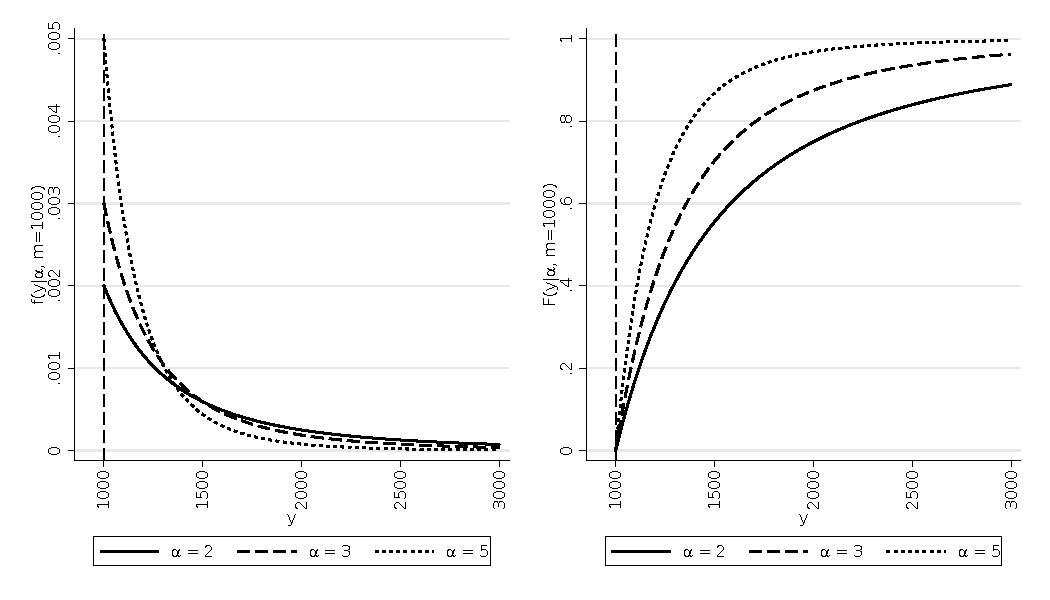
\includegraphics[width=\textwidth,height=3.125in]{./graphs/04_paretoDistGraphs.pdf}

\note{\begin{itemize}\tightlist

\item Here we can see how the Probability and Cumulative Distribution looks like.
\item - Only defined after lowerbound
\item - very heavy right tail 
\item - very left dense

\end{itemize}}

\end{frame}

\begin{frame}[fragile,fragile]{Graphical Visualisation II}
\protect\hypertarget{graphical-visualisation-ii}{}

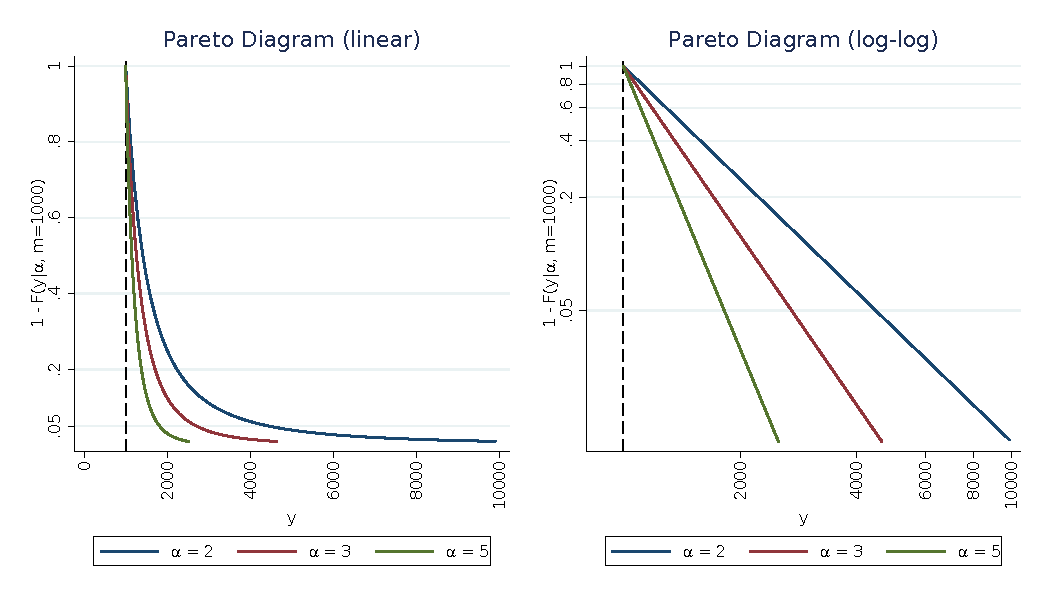
\includegraphics[width=\textwidth,height=3.125in]{graphs/04_paretoDiagram.pdf}

\note{\ttfamily{
In order to better visualise this distribution TWO transformations are taken:

1. calculate 1 - CDF\\
2. plot on log-log scale (or log-log the data)\\
\qquad .\\
\qquad .

HERE: lower bound = 1000 \\
\qquad $~~\alpha$ = Slope in loglog \\
\qquad - Approx. interpretation: for a percentage increase in $y$, the proportion of *richer* individuals by $\alpha$ percents (NOT PERCENTAGE POINTS).
}}

\end{frame}

\begin{frame}{Properties}
\protect\hypertarget{properties}{}

\emph{Pareto's \(\alpha\):}

\begin{itemize}
\tightlist
\item
  Approx. interpretation: for a percentage increase in \(y\), the
  proportion of \emph{richer} individuals by \(\alpha\) percents.
\item
  Higher \(\alpha\) values \(\Rightarrow\) less
  inequality.\footnote<.->{for inequality measures satisfying the
    \emph{Weak Transfers Principle} (Cowell 2011, p.~93).}
\item
  Several inequality indices can be estimated based on \(\alpha\).

  \begin{itemize}
  \tightlist
  \item
    Example: Gini coefficient: \(\frac{1}{2 \alpha - 1}\).
  \end{itemize}
\end{itemize}

\emph{Possible problems:}

\begin{itemize}
\tightlist
\item
  High flexibility on estimating the lower bound
\item
  Sensibility of \(\alpha\) due to choice of the lower bound
  \(\underline y\)
\end{itemize}

\note{
PROPERTIES
\begin{itemize}\tightlist
\item Interpretation
\item higher value --> less inequality
\item Inequality indices can be estimated based on $\alpha$
\item - - - GINI coef.

\end{itemize}

PROBLEMS
\begin{itemize}\tightlist
\item High flexibility on estimating the lower bound
\item Sensibility of $\alpha$ due to choice of the lower bound $\underline y$
\item For narrow excerpts of the data other distributions are "just as good"
\end{itemize}
}

\end{frame}

\end{document}
